\section{Relaciones}
Las relaciones son un concepto muy usado en computación, principalmente en el ámbito de las Bases de Datos (Bases de Datos Relacionales).
Intuitivamente una relación matemática puede verse como una \emph{correspondencia} de objetos de distintos dominios.
Generalmente en el contexto de Bases de Datos, esta correspondencia está dada por una tabla.
Por ejemplo la siguiente tabla muestra un trozo de la correspondencia entre alumnos y los cursos que ellos están tomando durante este semestre:
\begin{center}
\begin{tabular}{l|l}
{\bf Alumno} & {\bf Curso} \\ \hline
Aliaga & Lenguajes Formales \\
Aliste & Modelos Discretos \\
Aliste & Algoritmos y Estructuras de Datos \\
Arias &  Modelos Discretos \\
Arias &  Algoritmos y Estructuras de Datos \\
Acevedo & Algotimos y Estructuras de Datos \\
Bravo & Lenguajes Formales \\
\vdots & \vdots
\end{tabular}
\end{center}
Esta correspondencia nos dice por ejemplo que el alumno Aliaga está tomando el curso de Lenguajes Formales y que el alumno Aliste está tomando el curso de Modelos Discretos y de Algoritmos y Estructuras de Datos.

En esta sección formalizaremos el concepto de relación matemática y veremos diversas aplicaciones de él.

Lo primero que se debe definir para estudiar relaciones es el concepto de par ordenado:

\begin{definicion}
Se define el \emph{par ordenado} $(a,b)$ de los elementos $a$ y $b$ ambos elementos de un conjunto universal $\U$, de la siguiente manera:
\[
(a,b)=\{\{a\},\{a,b\}\}.
\]
La idea detrás de esta definición es que dos pares ordenados son iguales si y sólo si sus \emph{componentes} son iguales por separado, es decir:
\[
(a,b)=(c,d)\text{ si y sólo si }a=c\wedge b=d.
\]
Como ejercicio se puede demostrar esta propiedad a partir de la definición.
\end{definicion}
Esta definición se puede extender para soportar \emph{tríos ordenados} $(a,b,c)=((a,b),c)$, \emph{cuadruplas ordenadas} $(a,b,c,d)=((a,b,c),d)$ y en general, $n$--tuplas ordenadas $(a_1,a_2,\ldots,a_n)=((a_1,a_2,\ldots,a_{n-1}),a_n)$.
La siguiente definición importante en el contexto de las relaciones matemáticas es la de producto cartesiano.

\begin{definicion}
Sea $A$ y $B$ conjuntos subconjuntos de un conjunto universal $\U$, se define el \emph{producto cartesiano} entre $A$ y $B$, $A\times B$ como
\[
A\times B=\{(a,b)\;|\;a\in A\wedge b\in B\},
\]
o sea, $A\times B$ es el conjunto de todos los pares ordenados tales que su primera componente está en $A$ y su segunda en $B$.
\end{definicion}
Esta definición también se puede extender al producto cartesiano entre varios conjuntos, $A_1\times A_2\times\cdots\times A_n$.
Ahora podemos definir lo que es una relación:

\begin{definicion}
Sean $A$ y $B$ conjuntos, $R$ es una \emph{relación binaria} de $A$ en $B$ si 
\[
R\subseteq A\times B.
\]
Similarmente $R$ se dice una relación binaria \emph{sobre} $A$ si
\[
R\subseteq A\times A.
\]
\end{definicion}

\begin{ejemplo}
Supongamos que $A$ es el conjunto de todos los nombres de alumnos de la carrera de computación y que $B$ es el conjuntos de todos los nombres de cursos de computación, entonces la tabla que relaciona cada alumno con los cursos que está tomando este semestre es una relación binaria de $A$ en $B$.
Llamemos ${\it CargaComp}$ a esa relación, es claro que ${\it CargaComp}\subseteq A\times B$.
De hecho en $A\times B$ aparecen todos los pares posibles de nombres de alumnos y nombres de cursos, sin embargo en ${\it CargaComp}$ aparecen sólo aquellas en las que el alumno pertenece al curso en este semestre.
Por ejemplo, el par 
\[
(\text{Aliste, Lenguajes Formales})\in A\times B,
\]
sin embargo 
\[
(\text{Aliste, Lenguajes Formales})\notin {\it CargaComp}.
\]
\end{ejemplo}

Es posible extender el concepto de relación binaria a relación $n$--aria sobre más de dos conjuntos.
$R$ es una relación $n$--aria si $R\subseteq A_1\times A_2\times\cdots\times A_n$.
De hecho este es mucho más el caso que ocurre en las bases de datos.
Es muy común tener por ejemplo una tabla con información de personas que relacionan el RUT de una persona, con su nombre, teléfono, dirección, edad, etc.

En nuestro estudio estaremos generalmente interesados en relaciones binarias casi siempre sobre un único conjunto.
Para una relación binaria $R$, si el par $(a,b)$ está relacionado por $R$, o sea $(a,b)\in R$, escribiremos también $aRb$, de la misma manera si el par no está relacionado escribiremos $a\nr Rb$.
Esta notación debiera ser familiar para el alumno por ejemplo en relaciones de desigualdad, de hecho para un par que está relacionado por la relación \emph{menor o igual} no escribimos $(a,b)\in\leq$ si no más bien $a\leq b$, y si el par no está relacionado escribimos $a\not\leq b$.

\begin{ejemplo}
\begin{enumerate}
  \itemsep 0pt
  \item Sea $A=\{a,b,c,d,e\}$ entonces el siguiente conjunto es una relación sobre $A$.
  \[
  R=\{(a,b),(b,b),(b,c),(c,b),(c,d),(d,a),(d,b),(d,c),(d,d),(d,e)\}.
  \]
  Decimos por ejemplo que $aRb$, $dRc$, $a\nr Rd$ y $c\nr Re$.
  \item
	La relación \emph{divide a}, denotada por $|$, sobre los naturales sin el $0$, es una relación tal que $a$ está relacionado con $b$ si y sólo si $b$ es un múltiplo de $a$,
	\[
	%|\subseteq(\N-\{0\})\times(\N-\{0\}),\hspace*{3em}
	a|b\text{ si y sólo si }\exists k\in\N\text{ tal que }b=ka.
	\]
	Entonces sabemos que $3|9$ y que $18|72$ pero que $7\hspace*{-0.5em}\not |9$.
	Algo más que podríamos decir es que, por ejemplo, $1$ y $17$ son los únicos naturales relacionado \emph{por la izquierda} con $17$ (>por qué?).
	
	\item
	La relación \emph{equivalencia módulo $n$} con $n\in\N$, que denotaremos por $\equiv_n$, sobre los naturales, es una relación tal que $a$ está relacionado con $b$ si y sólo si $|a-b|$ es múltiplo de $n$.
	\[
	%\equiv_n\subseteq \N\times\N,\hspace*{3em}
	a\equiv_nb\text{ si y sólo si }\exists k\in\N\text{ tal que }|a-b|=kn.
	\]
	Entonces si por ejemplo $n=7$, sabemos que $2\equiv_723$, $8\equiv_71$, $19\not\equiv_74$.
	Algo más que podríamos decir es que por ejemplo, para todo $n\in\N$ se cumple que $0\equiv_nn$.
	
	\item
	Sea $\U$ un conjunto cualquiera y sea $C\subseteq\U$ un subconjunto fijo de $\U$.
	Podemos definir la relación $\mathcal R_C$ sobre $\P(\U)$ (el conjunto potencia de $\U$), tal que $A$ está relacionado con $B$, si y sólo si $A$ y $B$ tienen los mismos elementos en común con $C$.
	\[
	%\mathcal R_C\subseteq\P(\U)\times\P(\U),\hspace*{3em}
	A\mathcal R_CB\text{ si y sólo si }A\cap C=B\cap C.
	\]
	Podríamos decir por ejemplo que $\forall X\in\P(\U)$, si $X\cap C=\emptyset$ entonces $XR_C\emptyset$.
	Además, si $CR_CX$ entonces necesariamente se cumple que $C\subseteq X$.
\end{enumerate}
\end{ejemplo}

\subsection{Propiedades de las Relaciones Binarias}
\label{sec:prop-rel}
\begin{definicion}
Sea $R$ una relación sobre un conjunto $A$.
$R$ se dice:
\begin{itemize}
	\item 
	\emph{Refleja} (o \emph{reflexiva}) si para todo $x\in A$, $x$ está relacionado con $x$ mediante $R$.
	\[
	R\text{ es refleja si y sólo si }\forall x\in A\text{ se cumple que }xRx
	\]
	
	\item
	\emph{Simétrica} si cada vez que el par $(x,y)$ está relacionado por $R$, el par $(y,x)$ también lo está.
	\[
	R\text{ es simétrica si }xRy\Rightarrow yRx
	\]
	
	\item
	\emph{Asimétrica} si cada vez que el par $(x,y)$ está relacionado por $R$, el par $(y,x)$ no está relacionado por $R$.
	\[
	R\text{ es asimétrica si }xRy\Rightarrow y\nr Rx
	\]
	
	\item
	\emph{Antisimétrica} si la única forma de que los pares $(x,y)$ e $(y,x)$ estén relacionados, es cuando $x=y$.
	\[
	R\text{ es antisimétrica si }xRy\wedge yRx\Rightarrow x=y
	\]
	
	\item
	\emph{Transitiva} si cada vez que los pares $(x,y)$ e $(y,z)$ están relacionados, entonces el par $(x,z)$ también está relacionado por $R$.
	\[
	R\text{ es transitiva si }xRy\wedge yRz\Rightarrow xRz
	\]
\end{itemize}
\end{definicion}
\begin{ejemplo}
\begin{enumerate}
  \itemsep 0pt
  \item La relación $|$ es refleja, antisimétrica y transitiva.
  Demostraremos las propiedades de antisimetría y transitividad, la reflexividad se deja como ejercicio.
  
  Para demostrar antisimetría, debemos probar que si ocurre que $a|b$ y $b|a$ entonces necesariamente $a=b$.
  Supongamos que $a|b$, entonces sabemos que existe un $k_1\in\N$ tal que $k_1a=b$, por otro lado, si además $b|a$ entonces sabemos que existe un $k_2\in\N$ tal que $k_2b=a$.
  De estas dos igualdades obtenemos $k_1k_2b=b$ de donde concluimos que
  \[
  k_1k_2=1\hspace*{3em}\text{con }k_1,k_2\in\N.
  \]
  La única forma de que esto sea cierto para dos naturales es que ambos sean $1$, por lo que necesariamente $a=b$.
  Hemos demostrado que $a|b\wedge b|a\Rightarrow a=b$.
  
  Demostraremos ahora transitividad.
  Supongamos que $a|b$ y que $b|c$, por definición sabemos que existen $k_1,k_2\in\N$ tales que $k_1a=b$ y $k_2b=c$.
  Uniendo estas últimas igualdades obtenemos $k_1k_2a=c$, y ya que $k_1k_2\in\N$ concluimos que $a|c$.
  Hemos demostrado que $a|b\wedge b|c\Rightarrow a|c$.
  
  \item 
 	La relación $\equiv_n$ es refleja, simétrica y transitiva.
 	Demostraremos sólo la transitividad, las otras propiedades se dejan como ejercicio.
 	Supongamos que $x\equiv_ny$ y que $y\equiv_nz$, entonces existen $k_1,k_2\in\N$ tales que $|x-y|=k_1n$ y $|y-z|=k_2n$.
 	Dependiendo de los valores de $x,y$ y $z$ se pueden dar cuatro casos:
 	\[
 	\begin{array}{rr}
 	x-y=k_1n & y-z=k_2n \\
 	x-y=-k_1n & y-z=-k_2n
 	\end{array}
 	\]
 	trataremos de analizar los cuatro simultáneamente.
 	Sea $y-z=\pm k_1n$, por lo que $y=\pm k_1n+z$, reemplazando en la otra igualdad obtenemos $x-(\pm k_1n+z)=\pm k_2n$ de donde se concluye que 
 	\[
 	x-z=(\pm k_1+\pm k_2)n. 
 	\]
 	Si tomamos valor absoluto a esta última igualdad obtenemos
 	\[
 	|x-z|=|\pm k_1+\pm k_2|n
 	\]
 	de donde si $k_3=|\pm k_1+\pm k_2|$, $k_3\in\N$ y $|x-z|=k_3n$ y por lo tanto $x\equiv_nz$.
 	
 	\item La relación $R_C$ definida en el ejemplo anterior, es refleja, simétrica y transitiva.
 	Las demostraciones resultan directas de las propiedades del operador $\cap$ y se dejan como ejercicio.
\end{enumerate}
\end{ejemplo}

Se pueden definir distintos tipos de relaciones según las propiedades que estas tengan.
Más adelante estudiaremos dos tipos muy importantes.

\subsection{Representación Matricial}
Si tenemos una relación $R$ sobre un conjunto finito $A$, esta puede representarse mediante una matriz binaria (con sólo ceros y unos).
Esta representación es muy conveniente si queremos que un computador procese información, opere relaciones o decida propiedades acerca de la relación.
Para obtener la representación, etiquetamos tanto las columnas como filas de la matriz con elementos de $A$ en algún orden arbitrario.
Un $1$ en la posición $(i,j)$ de la matriz indica que los elementos correspondientes a la fila $i$ columna $j$ están relacionados, un $0$ en cambio india que no están relacionados.
Generalmente a la matriz que representa a la relación $R$ la llamaremos $M_R$.

\begin{ejemplo}
Sea $A=\{a,b,c,d,e\}$, el siguiente conjunto es una relación sobre $A$.
  \[
  R=\{(a,b),(b,b),(b,c),(c,b),(c,d),(d,a),(d,b),(d,c),(d,d),(d,e)\}.
  \]
  La matriz que representa a $R$ es
  \[
  M_R=
  \left[
  \begin{array}{c c c c c}
  0 & 1 & 0 & 0 & 0 \\
  0 & 1 & 1 & 0 & 0 \\
  0 & 1 & 0 & 1 & 0 \\
  1 & 1 & 1 & 1 & 1 \\
  0 & 0 & 0 & 0 & 0 
  \end{array}\right]
  \]
  en donde las filas y columnas se han etiquetado en orden alfabético.
\end{ejemplo}

>Cómo puedo de forma simple analizando la matriz $M_R$ determinar si $R$ es refleja, simétrica, etc.?
No es difícil notar que $R$ es refleja si y sólo si $M_R$ tiene toda la diagonal con $1$'s y que es simétrica si $M_R=(M_R)^T$.
Para formalizar estas nociones intuitivas introduciremos ciertos conceptos.

\begin{definicion}
Sean $R$ y $S$ dos relaciones sobre el conjunto finito $A$ de $n$ elementos, y $M_R$ y $M_S$ las matrices representantes respectivamente.
Llamaremos $[M_R]_{(i,j)}$ a la componente $(i,j)$ de la matriz $M_R$.
\begin{enumerate}
  \itemsep 0pt
  \item Diremos que $M_R$ es menor o igual a $M_S$ y escribiremos $M_R\leq M_S$ si para todo par $(i,j)$ se cumple que $[M_R]_{(i,j)}\leq[M_S]_{(i,j)}$.
  Note que $M_R\leq M_S$ si y sólo si cada vez que $[M_R]_{(i,j)}=1$ entonces ocurre que $[M_S]_{(i,j)}=1$, $M_S$ tiene $1$'s al menos en todas las posiciones en que $M_R$ tiene $1$'s (y posiblemente en otras posiciones más).
  \item Definimos la \emph{disyunción} o suma lógica $M_R\vee M_S$ como la matriz cuyas componentes cumplen 
  \[
  [M_R\vee M_S]_{(i,j)}=\left\{
  						\begin{array}{lr}
  						1 & \text{ si }[M_R]_{(i,j)}=1\text{ o }[M_S]_{(i,j)}=1 \\
  						0 & \text{ en otro caso.}
  						\end{array}\right.
  \]
  \item Definimos la \emph{conjunción} $M_R\wedge M_S$ como la matriz cuyas componentes cumplen
  \[
  [M_R\wedge M_S]_{(i,j)}=\left\{
  						\begin{array}{lr}
  						1 & \text{ si }[M_R]_{(i,j)}=1\text{ y }[M_S]_{(i,j)}=1 \\
  						0 & \text{ en otro caso.}
  						\end{array}\right.
  \]
  \item Definiremos la multiplicación $M_R\cdot M_S$ como la matriz cuyas componentes se forman al multiplicar ambas matrices de la manera usual del álgebra de matrices,
  \[
  [M_R\cdot M_S]_{(i,j)}=\sum_{l=1}^n[M_R]_{(i,l)}[M_S]_{(l,j)}
  \] 
  pero suponiendo suma booleana, es decir, suponiendo que $1+1=1$.
  De la misma manera podemos definir la potencia $(M_R)^k=M_R\cdot M_R\cdots$ ($k$ veces) $\cdots M_R$.
\end{enumerate}
\end{definicion}

Ahora podemos establecer más formalmente las definiciones intuitivas

\begin{teorema}
\label{teo:propiedades-matrices-relaciones}
Sea $R$ una relación sobre un conjunto $A$ de $n$ elementos y sea $M_R$ la matriz que representa a $R$.
Sea $I_n$ la matriz identidad de $n\times n$.
Se cumple que:
\begin{enumerate}
  \itemsep 0pt
  \item $R$ es refleja si y sólo si $I_n\leq M_R$.
  \item $R$ es simétrica si y sólo si $M_R=(M_R)^T$.
  \item $R$ es antisimétrica si y sólo si $M_R\wedge (M_R)^T\leq I_n$
  \item $R$ es transitiva si y sólo si $M_R\cdot M_R=(M_R)^2\leq M_R$
\end{enumerate}
\begin{demostracion}
A modo de ejemplo demostraremos las propiedades 2 y 4, las otras se dejan como ejercicio:
\begin{enumerate}
  \itemsep 0pt
  \stepcounter{enumi}
  \item Sean $x,y\in A$ y tal que se les han asignado las posiciones $i$ y $j$ dentro de $M_R$ respectivamente.
  
  ($\Leftarrow$) Supongamos que $xRy$ esto implica que $[M_R]_{(i,j)}=1$, dado que que $M_R=(M_R)^T$ tenemos que $[M_R]_{(j,i)}=1$ de donde resulta que $yRx$, por lo que $R$ es simétrica.
  
  ($\Rightarrow$) Supongamos que $[M_R]_{(i,j)}=1$, esto implica que $xRy$, dado que $R$ es simétrica necesariamente $yRx$ por lo que $[M_R]_{(j,i)}=1$. 
  Supongamos ahora que $[M_R]_{(i,j)}=0$, esto implica que $x\nr Ry$ y dado que $R$ es simétrica necesariamente $y\nr Rx$ por lo que $[M_R]_{(j,i)}=0$.
  De los dos argumentos anteriores se concluye que $M_R=(M_R)^T$.
  
  \stepcounter{enumi}
  \item Sean $x,y,z\in A$ y tal que se les han asignado las posiciones $i$, $k$ y $j$ dentro de $M_R$ respectivamente.
  
  ($\Leftarrow$) Sean $x,y,z\in A$ tal que se les han asignado las posiciones $i$, $k$ y $j$ dentro de $M_R$ respectivamente.
  Supongamos que $xRy$ y que $yRz$, por lo que $[M_R]_{(i,k)}=[M_R]_{(k,j)}=1$.
  Analicemos la posición $[(M_R)^2]_{(i,j)}$, esta se forma a partir de la multiplicación $[(M_R)^2]_{(i,j)}=\sum_{l=1}^n[M_R]_{(i,l)}[M_R]_{(l,j)}$, que tiene valor $1$ ya que $[M_R]_{(i,k)}=[M_R]_{(k,j)}=1$.
  Ahora, dado que $(M_R)^2\leq M_R$ necesariamente $[M_R]_{(i,j)}=1$ de donde se concluye que $xRz$.
  Hemos demostrado que cada vez que se cumple $xRy \wedge yRz$ se concluye que $xRz$, por lo tanto $R$ es transitiva.
  
  ($\Rightarrow$) Supongamos que a $x,y\in A$ se les han asignado las posiciones $i$ y $j$ dentro de $M_R$.
  Supongamos ahora que $[(M_R)^2]_{(i,j)}=1$, esto ocurre si y sólo si $\sum_{l=1}^n[M_R]_{(i,l)}[M_R]_{(l,j)}=1$ que ocurre si y sólo si existe un $l$ tal que $[M_R]_{(i,l)}=[M_R]_{(l,j)}=1$, o sea, si y sólo si existe un $v\in A$ tal que $xRv$ y $vRy$.
  Como estamos suponiendo que $R$ es transitiva, necesariamente $xRy$ por lo que $[M_R]_{(i,j)}=1$.
  Demostramos que cada vez que $[(M_R)^2]_{(i,j)}=1$ se cumple que $[M_R]_{(i,j)}=1$ de donde concluimos que $(M_R)^2\leq M_R$.
\end{enumerate}
\end{demostracion}
\end{teorema}

Existe una intima relación entre los operadores matriciales definidos y los operadores de relaciones sobre conjuntos finitos.
Antes de enunciar el siguiente teorema, necesitamos un par de definiciones:

\begin{definicion}
%\begin{enumerate}
%\item 
Sea $R$ una relación binaria de $A$ en $B$.
La \emph{inversa} de $R$, denotada por $R^{-1}$, es la relaón de $B$ en $A$ definida por
  $$
  R^{-1}=\{(x,y)\in B\times A\;|\; yRx\}.
  $$
%  \item 

Sea $R$ una relación binaria de $A$ en $B$ y $S$ una 
  relación binaria de $B$ en $C$.
  La \emph{composición} entre $R$ y $S$, denotada por $R\circ S$,
  es la relación de $A$ en $C$ definida por
  $$
  R\circ S=\{(x,z)\in A\times C\;|\;\text{ existe un }y\in B\text{ tal que }xRy\text{ e }ySz\}.
  $$
%  \end{enumerate}
\end{definicion}

El siguiente teorema relaciona propiedades de las matrices que representan relaciones
y propiedades y operaciones sobre las relaciones mismas.

\begin{teorema}
Sean $R$ y $S$ dos relaciones sobre un conjunto $A$ con $n$ elementos, y $M_R$ y $M_S$ respectivamente las matrices que las representan, entonces se cumple que: \label{teo:operadores-matriz-relacion}
\begin{enumerate}
  \itemsep 0pt
  \item $R\subseteq S$ si y sólo si $M_R\leq M_S$.
  \item La matriz que representa a la relación $R\cup S$ es $M_R\vee M_S$.
  \item La matriz que representa a la relación $R\cap S$ es $M_R\wedge M_S$.
  \item La matriz que representa a $R^{-1}$ es $(M_R)^T$.
  \item La matriz que representa a $R\circ S$ es $M_R\cdot M_S$.
\end{enumerate}
\begin{demostracion} Ejercicio.
\end{demostracion}
\end{teorema}

Se debe tener cuidado con la aplicabilidad de este teorema ya que sólo tiene sentido representar una relación usando matrices cuando esta está definida sobre un conjunto finito.
>Podemos establecer propiedades como en el teorema~\ref{teo:propiedades-matrices-relaciones} para determinar cuándo una relación cualquiera (no necesariamente definida sobre un conjunto finito) cumple con las propiedades de reflexividad, simetría, etc.? 
La respuesta es sí, de hecho el siguiente teorema establece estas propiedades.

\begin{teorema}
\label{teo:propiedades-relaciones}
Sea $R$ una relación cualquiera sobre un conjunto $A$ no necesariamente finito, y sea $D$ la \emph{relación diagonal} definida por $D=\{(x,x)\;|\; x\in A\}$, entonces se cumple que:
\begin{enumerate}
  \itemsep 0pt
  \item $R$ es refleja si y sólo si $D\subseteq R$.
  \item $R$ es simétrica si y sólo si $R=R^{-1}$.
  \item $R$ es antisimétrica si y sólo si $R\cap R^{-1}\subseteq D$.
  \item $R$ es transitiva si y sólo si $R\circ R\subseteq R$.
\end{enumerate}
\begin{demostracion}
Alguien podría estar tentado a argumentar que el teorema es una conclusión directa de los dos teoremas anteriores, esta sería una argumentación correcta sólo en el caso de que la relación estuviese definida sobre un conjunto finito.
Sin embargo este no es el caso, $A$ no necesariamente es finito, por lo que debe entregarse otro argumento.
A modo de ejemplo demostraremos la propiedad 3, las demás se dejan como ejercicio.
\begin{enumerate}
  \itemsep 0pt
  \stepcounter{enumi}
  \stepcounter{enumi}
  \item ($\Leftarrow$) Supongamos que $xRy\wedge yRx$, esto implica que $xRy\wedge xR^{-1}y$ por la definición de $R^{-1}$, y que por lo tanto $(x,y)\in R\cap R^{-1}$.
  Ahora dado que $R\cap R^{-1}\subseteq D$, necesariamente $(x,y)\in D$ de donde se deduce que $x=y$ (es la única forma de que $(x,y)\in D$).
  Hemos demostrado que si $xRy\wedge yRx$ entonces $x=y$ y por lo tanto $R$ es antisimétrica.
  
  ($\Rightarrow$) Sea $(x,y)\in R\cap R^{-1}$ esto implica que $xRy\wedge xR^{-1}y$ y que por lo tanto $xRy\wedge yRx$ por la definición de $R^{-1}$.
  Ahora, dado que $R$ es antisimétrica, si $xRy\wedge yRx$ entonces necesariamente $x=y$ y por lo tanto $(x,y)\in D$.
  Hemos demostrado que si $(x,y)\in R\cap R^{-1}$ entonces $(x,y)\in D$, luego se cumple que $R\cap R^{-1}\subseteq D$.
\end{enumerate}
\end{demostracion}

Nótese que, a pesar de que este teorema no puede establecerse como conclusión a partir de los dos teoremas anteriores (teoremas~\ref{teo:propiedades-matrices-relaciones} y~\ref{teo:operadores-matriz-relacion}), usando este teorema y el teorema~\ref{teo:operadores-matriz-relacion} se concluye inmediatamente el teorema~\ref{teo:propiedades-matrices-relaciones}.
Por ejemplo, dado que para cualquier relación $R$, esta es simétrica si y sólo si $R=R^{-1}$, entonces si $R$ es una relación definida sobre un conjunto finito, dado que $M_{R^{-1}}=(M_R)^T$, $R$ será simétrica si y sólo si $M_R=(M_R)^T$ que es la propiedad 2 del teorema~\ref{teo:propiedades-matrices-relaciones}.
Como ejercicio intente dar una demostración para las demás propiedades del teorema~\ref{teo:propiedades-matrices-relaciones} usando esta idea. 
%\footnote{En el teorema~\ref{teo:propiedades-matrices-relaciones} se usa la matriz $I_n$ para establecer algunas propiedades, note que si $D$ es la relación diagonal sobre un conjunto de $n$ elementos, entonces $M_D=I_n$.}.
\end{teorema}

\subsection{Clausuras}
Muchas veces en computación nos encontramos con relaciones que no cumplen cierta propiedad pero que nos gustaría que la cumplieran para poder obtener información adicional.
En el siguiente ejemplo se motiva este tema.

\begin{ejemplo}
Supongamos que se tiene la siguiente tabla de vuelos directos entre el conjunto $\{$Stgo, BsAs, Miami, Lond, Frnk, Paris, Mosc$\}$ de ciudades del mundo:
\begin{center}
\begin{tabular}{l|l} 
Origen & Destino \\ \hline
Stgo & BsAs \\
Stgo & Miami \\
Stgo & Lond \\
BsAs & Stgo \\
Miami & Stgo \\
Miami & Lond \\
Lond & Stgo \\
Lond & Paris \\
Frnk & Paris \\
Frnk & Mosc \\
Paris & Mosc \\
Mosc & Frnk 
\end{tabular}
\end{center}
Por ejemplo la tabla nos dice que existe un vuelo directo desde Stgo a BsAs y que también existe un vuelo directo desde BsAs a Stgo.
Esto no siempre ocurre, por ejemplo, existe un vuelo directo entre Miami y Lond pero no existe uno entre Lond y Miami.
Es claro que si existe un vuelo directo desde Lond a Stgo y uno desde Stgo a BsAs, entonces es posible llegar desde Lond a BsAs haciendo escala en Stgo.
La pregunta entonces es, dada la relación de vuelos directos >cómo se puede obtener una relación que me indique todos los pares de ciudades tales que existe un vuelo no necesariamente directo, posiblemente con escalas, desde una a la otra?
En lo que sigue de la sección definiremos este problema.
%Si quisiéramos representar esta relación usando una matriz resultaría:
%\[
%M=\left[\begin{array}{ccccccc}
%0 & 1 & 1 & 1 & 0 & 0 & 0 \\
%1 & 0 & 0 & 0 & 0 & 0 & 0 \\
%1 & 0 & 0 & 1 & 0 & 0 & 0 \\
%1 & 0 & 0 & 0 & 0 & 1 & 0 \\
%0 & 0 & 0 & 0 & 0 & 1 & 1 \\
%0 & 0 & 0 & 0 & 0 & 0 & 1 \\
%0 & 0 & 0 & 0 & 1 & 0 & 0 
%\end{array}
%\right]
%\]
\end{ejemplo}
\begin{definicion}
Sea $\varphi$ una propiedad de relaciones sobre un conjunto $A$ (no necesariamente finito), y sea $R$ una relación cualquiera sobre $A$.
Se define la \emph{clausura} $\varphi$ de $R$ como la menor relación que contiene a $R$ y que cumple la propiedad $\varphi$.
Hablaremos de la \emph{clausura refleja} de $R$, \emph{clausura simétrica} de $R$ y \emph{clausura transitiva} de $R$, y la llamaremos $CR(R)$, $CS(R)$ y $CT(R)$ respectivamente.

En la definición aparece el concepto de ``menor relación'', en este contexto menor es con respecto a la relación $\subseteq$, se refiere a que por ejemplo, si $CT(R)$ es la clausura transitiva de $R$, para cualquier otra relación $T$ transitiva que contenga a $R$ se debe cumplir que $CT(R)\subseteq T$.
\end{definicion}

\begin{ejemplo}
En el ejemplo de vuelos directos anterior,
si existe un vuelo directo entre el par de ciudades $(C_1,C_2)$ y otro vuelo directo entre el par $(C_2,C_3)$ en la relación de vuelos posiblemente con escalas nos gustaría tener al par de ciudades $(C_1,C_3)$.
Ahora si por ejemplo también existe un vuelo directo entre el par $(C_3,C_4)$, nos gustaría tener a los pares de ciudades $(C_1,C_4)$ y $(C_2,C_4)$ en la relación de vuelos posiblemente con escalas.
Lo que necesitamos entonces es una relación que contenga a la de vuelos directos pero que además sea transitiva.
Además necesitamos una propiedad muy importante, que la nueva relación no contenga pares de ciudades ``de más'', de hecho no debiera contener el par $($Stgo, Mosc$)$.
La relación de vuelos posiblemente con escalas resulta ser una relación que contiene a la de vuelos directos, que es transitiva y que es la más chica posible, es decir, resulta ser la clausura transitiva de la relación de vuelos directos.

Dado que sabemos que lo que queremos es la clausura transitiva de la relación 
el siguiente paso es preguntarnos cómo podemos obtenerla.
Una posibilidad para enfrentar inicialmente el problema es mirar la matriz que representa a la relación.
En nuestro ejemplo, la matriz resulta ser
\[
M_{V}=\left[\begin{array}{ccccccc}
0 & 1 & 1 & 1 & 0 & 0 & 0 \\
1 & 0 & 0 & 0 & 0 & 0 & 0 \\
1 & 0 & 0 & 1 & 0 & 0 & 0 \\
1 & 0 & 0 & 0 & 0 & 1 & 0 \\
0 & 0 & 0 & 0 & 0 & 1 & 1 \\
0 & 0 & 0 & 0 & 0 & 0 & 1 \\
0 & 0 & 0 & 0 & 1 & 0 & 0 
\end{array}
\right]
\]
en donde las ciudades se han ordenado según su aparición en el conjunto del ejemplo.
Si ahora miramos la matriz al cuadrado obtenemos:
\[
M_V\cdot M_V=\left[\begin{array}{ccccccc}
1 & 0 & 0 & 1 & 0 & 1 & 0 \\
0 & 1 & 1 & 1 & 0 & 0 & 0 \\
1 & 1 & 1 & 1 & 0 & 1 & 0 \\
0 & 1 & 1 & 1 & 0 & 0 & 1 \\
0 & 0 & 0 & 0 & 1 & 0 & 1 \\
0 & 0 & 0 & 0 & 1 & 0 & 0 \\
0 & 0 & 0 & 0 & 0 & 1 & 1 
\end{array}
\right]
\]
$M_V\cdot M_V$ tiene un $1$ en la posición correspondiente al par (BsAs, Miami) el que aparece debido a que en $M_V$ había un $1$ en la posición correspondiente al par (BsAs, Stgo) y un $1$ en la posición correspondiente al par (Stgo, Miami).
Si miramos con más detención, nos daremos cuenta de que cada una de las posiciones que tienen $1$ en $M_V\cdot M_V$ corresponden a pares de ciudades $(C_1,C_2)$ tales que existe un vuelo con una escala intermedia entre $C_1$ y $C_2$.
De la misma forma de podría argumentar que $(M_V\cdot M_V)\cdot M_V$ contiene a todos los pares de ciudades tales que existe un vuelo con dos escalas intermedias entre ellas.
Entonces la matriz
$$M_V\vee(M_V)^2\vee(M_V)^3$$
corresponderá a una relación que tiene todos los pares de ciudades para los cuales existe un vuelo directo, o un vuelo con una escala intermedia, o un vuelo con dos escalas intermedias.
>Cuanto es el máximo número de escalas intermedias que se pueden tener en un vuelo entre un par de ciudades? 
La respuesta es simple, el vuelo más largo que se puede realizar es partir desde una ciudad, pasar por todas las otras ciudades y finalmente volver a la ciudad inicial, por lo que en nuestro caso la matriz
$$M_V\vee(M_V)^2\vee(M_V)^3\vee(M_V)^4\vee(M_V)^5\vee(M_V)^6\vee(M_V)^7$$
representaría a una relación que tiene todos los pares de ciudades $(C_1,C_2)$ para los cuales existe un vuelo posiblemente con escalas intermedias entre $C_1$ y $C_2$, o sea, representaría a la clausura transitiva de la relación de vuelos directos.

El siguiente teorema formaliza esta noción y la de otras clausuras.
\end{ejemplo}

%Dado que sabemos lo que queremos el siguiente paso es pensar en cómo lo obtenemos.
%El siguiente teorema nos entrega una forma de obtener clausuras de relaciones que se encuentran representadas usando matrices.
\begin{teorema}
\label{teo:clausuras-matrices-relaciones}
Sea $R$ una relación sobre un conjunto $A$ de $n$ elementos y sea $M_R$ la matriz que representa a $R$.
Entonces se cumple que:
\begin{enumerate}
  \itemsep 0pt
  \item La matriz que representa a la clausura refleja de $R$ es $$M_{CR(R)}=M_R\vee I_n.$$
  \item La matriz que representa a la clausura simétrica de $R$ es $$M_{CS(R)}=M_R\vee (M_R)^T.$$
  \item La matriz que representa a la clausura transitiva de $R$ es $$M_{CT(R)}=\bigvee_{i=1}^n(M_R)^i.$$ 
\end{enumerate}
\begin{demostracion}
La demostración es una conclusión directa del siguiente teorema que estudiaremos (teorema~\ref{teo:clausuras-relaciones}).
\end{demostracion}
\end{teorema}

Similarmente al teorema~\ref{teo:propiedades-relaciones} que nos daba una equivalencia entre las propiedades de las matrices que representan a una relación y las relaciones definidas no necesariamente sobre conjuntos finitos, podemos establecer un teorema que liga al anterior con clausuras de relaciones en general.

\begin{teorema}
\label{teo:clausuras-relaciones}
Sea $R$ una relación cualquiera sobre un conjunto $A$ no necesariamente finito, y sea $D$ la relación diagonal sobre $A$, entonces se cumple que:
\begin{enumerate}
  \itemsep 0pt
  \item La clausura refleja de $R$, $CR(R)$ se obtiene haciendo $$CR(R)=R\cup D.$$
  \item La clausura simétrica de $R$, $CR(R)$ se obtiene haciendo $$CS(R)=R\cup R^{-1}.$$
  \item La clausura transitiva de $R$, $CT(R)$ se obtiene haciendo $$CT(R)=\bigcup_{i=1}^{\infty}R^{i},$$
  donde $R^i$ representa a la composición $i$ veces $R$, es decir, inductivamente,
  $R^1=R$ y $R^{n+1}=R^{n}\circ R$.
\end{enumerate}
\begin{demostracion}
A modo de ejemplo demostraremos la propiedad 3, las demás se dejan como ejercicio.
\begin{enumerate}
  \itemsep 0pt
  \stepcounter{enumi}
  \stepcounter{enumi}
  \item Para demostrar que $\bigcup_{i=1}^{\infty}R^{i}$ es efectivamente igual a $CT(R)$ se deben demostrar tres cosas: (1) que $\bigcup_{i=1}^{\infty}R^{i}$ contiene a $R$, (2) que $\bigcup_{i=1}^{\infty}R^{i}$ es efectivamente transitiva y (3) que $\bigcup_{i=1}^{\infty}R^{i}$ es subconjunto de cualquier otra relación que contenga a $R$ y sea transitiva. % es subconjunto de .
  Demostraremos cada una por separado:
  \begin{itemize}
  	\itemsep 0pt
    \item[(1)] $\bigcup_{i=1}^{\infty}R^{i}=R\cup R^2\cup R^3\cup\cdots$ por lo que claramente $R\subseteq\bigcup_{i=1}^{\infty}R^{i}$.
    \item[(2)] Supongamos que el par $(x,y)$ e $(y,z)$ pertenecen a $\bigcup_{i=1}^{\infty}R^{i}$, demostraremos que entonces el par $(x,z)$ también pertenece a $\bigcup_{i=1}^{\infty}R^{i}$.
    Si $(x,y)\in\bigcup_{i=1}^{\infty}R^{i}$ entonces necesariamente $(x,y)\in R^j$ para algún $j$, de la misma manera sabemos que $(y,z)\in R^k$ para algún $k$.
    Por la definición de composición, sabemos entonces que el par $(x,z)\in R^j\circ R^k=R^{j+k}$ por lo que $(x,z)$ también pertenece a $\bigcup_{i=1}^{\infty}R^{i}$.
    \item[(3)] Sea $S$ una relación transitiva cualquiera tal que $R\subseteq S$, debemos demostrar que $\bigcup_{i=1}^{\infty}R^{i}\subseteq S$.
%, o sea, que si $(x,y)\in\bigcup_{i=1}^{\infty}R^{i}$ entonces también ocurre que $(x,y)\in S$.
    Demostraremos algo equivalente, demostraremos que para todo $i\geq 1$ se cumple que $R^i\subseteq S$ y por lo tanto $\bigcup_{i=1}^{\infty}R^{i}\subseteq S$.
    Lo haremos usando un argumento inductivo en $i$.
    La base se cumple por la definición de $S$, $R^1=R\subseteq S$.
    Ahora supongamos que $R^i\subseteq S$ y sea $(x,z)\in R^{i+1}$, demostraremos que entonces $(x,z)\in S$ y por lo tanto $R^{i+1}\subseteq S$.
    Si $(x,z)\in R^{i+1}$ entonces $(x,z)\in R^i\circ R$, lo que ocurre sólo si existe un $y$ tal que $(x,y)\in R^i\subseteq S$ e $(y,z)\in R\subseteq S$.
    Ahora dado que $S$ es transitiva y tenemos que $(x,y)\in S\wedge(y,z)\in S$ entonces necesariamente $(x,z)\in S$, por lo que $R^{i+1}\subseteq S$.
  \end{itemize}
\end{enumerate}
\end{demostracion}

Este teorema puede usarse para una demostración directa del teorema~\ref{teo:clausuras-matrices-relaciones}.
Por ejemplo, dado que para cualquier relación $R$ se cumple que $CS(R)=R\cup R^{-1}$ entonces si $R$ es una relación definida sobre un conjunto finito, se tiene que $M_{CS(R)}=M_R\vee M_{R^{-1}}=M_R\vee (M_R)^T$.
\end{teorema}

\subsection{Relaciones de Orden}

\begin{definicion}
Diremos que una relación binaria $R$ sobre un conjunto $A$ es una {\bf relación de orden parcial} si cumple con ser, refleja, antisimétrica y transitiva.
Generalmente cuando $R$ sea una relación de orden parcial la denotaremos por el símbolo $\preceq$.
Si $(x,y)\in\preceq$ o equivalentemente $x\preceq y$, diremos que ``$x$ es menor (o menor--igual) que $y$''.

Diremos además que, si $\preceq$ es una relación de orden parcial sobre $A$, entonces el par $(A,\preceq)$ es un orden parcial.
\end{definicion}

\begin{ejemplo}
\begin{enumerate}
  \itemsep 0pt
	\item Los pares $(\N,\leq)$, $(\Z,\leq)$, $(\R,\leq)$ son todas órdenes parciales.
  \item El par $(\N-\{0\},|)$ es un orden parcial.
  \item Sea $\U$ un conjunto fijo cualquiera, entonces $(\P(\U),\subseteq)$ es un orden parcial.
\end{enumerate}
La demostración de cada una de estas propiedades se deja como ejercicio.
\end{ejemplo}

%\begin{definicion}
%Para cada orden parcial $(A,\preceq)$ existe un orden parcial asociado, $(A,\preceq^{-1})$ el {\bf orden inverso} de $\preceq$.
%Al orden inverso de $\preceq$ lo llamaremos $\succeq$.
%\end{definicion}

>Por qué orden {\bf parcial}?
Parcial, en contraposición a total.
Estamos acostumbrados en los órdenes sobre $\N$, $\Z$ o $\R$, que si no se cumple que $x\leq y$ entonces necesariamente $y\leq x$.
Esto no ocurre en un orden parcial cualquiera, de hecho en el orden $(\N-\{0\},|)$ no ocurre ni que $6|9$ ni que $9|6$.
Tampoco en $(\P(\U),\subseteq)$, de hecho es totalmente posible encontrar un par de conjunto $A$ y $B$ tales que $A\not\subseteq B$ y $B\not\subseteq A$.
Esto motiva la siguiente definición.

\begin{definicion}
Diremos que $(A,\preceq)$ es un {\bf orden total (o lineal)} si es un orden parcial y para cada par de elementos $x,y\in A$ ocurre que $x\preceq y$ o que $y\preceq x$.
\end{definicion}

Cuando hablamos de órdenes parciales (o totales) sobre un conjunto estamos implícitamente estableciendo una estructura sobre el conjunto.
Nos gustaría poder hablar de elementos menores que, mayores que, máximos, mínimos, etc.
Las siguientes definiciones nos hablan de esto:

\begin{definicion}
Sea $(A,\preceq)$ un orden parcial, y sea $S\subseteq A$ un subconjunto no vacio cualquiera de $A$.
Sea $x$ un elemento cualquiera de $A$.
Diremos que:
\begin{enumerate}
	\itemsep 0pt
  \item $x$ es una \emph{cota inferior} de $S$ si para todo $y\in S$ se cumple que $x\preceq y$.
  %de manera similar $x$ será una \emph{cota superior} si para todo $y\in S$ se cumple que $y\preceq x$.
  \item $x$ es un \emph{elemento minimal} de $S$, si $x\in S$ y para todo $y$ en $S$ se cumple que $y\preceq x\Rightarrow y=x$, o sea, $x$ es minimal, si pertenece a $S$ y ningún elemento de $S$ es menor que $x$.
  %De manera similar, $x$ será un \emph{elemento maximal} si $x\in S$ para todo $y$ en $S$ se cumple que $x\preceq y\Rightarrow y=x$.
  \item $x$ es un \emph{mínimo} en $S$, si $x\in S$ y $x$ es cota inferior de $S$.
\end{enumerate}
De manera similar se pueden definir los conceptos de cota superior, elemento maximal, y máximo, por ejemplo, diremos que $x$ es una \emph{cota superior} de $S$ si para todo $y\in S$ se cumple que $y\preceq x$.
\end{definicion}

\begin{ejemplo}
\begin{enumerate}
	\item
	Sea el orden parcial $(\N-\{0\},|)$ y sea $S=\{2,3,5,10,15,20\}\subseteq \N$.
	Podemos decir por ejemplo que $1$ es una cota inferior para $S$, pero que $2$ no es una cota inferior (ya que $2$ no divide a $5$ ni a $15$).
	Podemos decir que $60$ es una cota superior para $S$, ya que $2|60$, $3|60, \ldots, 20|60$, y también $120$ es cota superior.
	$S$ tiene ademas, tres elementos minimales, $2$, $3$ y $5$, y tres elementos maximales $10$, $15$ y $20$.
	Finalmente podemos decir que $S$ no tiene ni mínimo ni máximo.
	>Podemos encontrar un $S\subseteq \N$ tal que todos sus elementos sean maximales y minimales a la vez?
	
	\item 
	Sea el orden parcial $(\P(\{1,2,3,4\}),\subseteq)$ y sea $\mathcal S=\{\{1\},\{1,2\},\{1,3\},\{1,2,3,4\}\}$.
	Podemos decir que $\{1\}$ es una cota inferior, un elemento minimal y un mínimo de $\mathcal S$, y que $\{1,2,3,4\}$ es una cota superior, un elemento maximal y un máximo de $\mathcal S$.
	Otra cota inferior para $\mathcal S$ es $\emptyset$.
	>Podemos encontrar un $\mathcal S\subseteq\P(\{1,2,3,4\})$ tal que todos sus elementos sean maximales y minimales a la vez?
	\end{enumerate}
\end{ejemplo}

\begin{teorema}
Sea $(A,\preceq)$ un orden parcial, y sea $S\subseteq A$ un subconjunto no vacio de $A$.
Si $S$ tiene un elemento mínimo, este es único.

\begin{demostracion}
Supongamos que existen dos elementos mínimos para $S$, digamos $s_1$ y $s_2$.
Dado que son mínimo, tanto $s_1,s_2\in S$ y además se cumple que $s_1\preceq s_2$ y que $s_2\preceq s_1$.
Dado que $\preceq$ es una relación de orden se concluye que $s_1=s_2$ (por antisimetría) y por lo tanto el mínimo es único.
\end{demostracion}

De la misma manera se puede establecer que el máximo de un conjunto es único.
Este teorema nos permite además hablar de él mínimo o él máximo de un conjunto $S$, que anotaremos como $\min(S)$ y $\max(S)$.
\end{teorema}

Note que el teorema dice ``Si $S$ tiene un elemento mínimo...'' esto porque ya vimos en los ejemplos que pueden existir conjuntos sin elementos mínimos.
La siguiente definición extiende el concepto de elemento mínimo.

\begin{definicion}
Sea $(A,\preceq)$ un orden parcial, y sea $S\subseteq A$ un subconjunto cualquiera de $A$.
Sea $x$ un elemento cualquiera de $A$.
Diremos que $s$ es un \emph{ínfimo} de $S$ si $s$ es una cota inferior  de $S$ y para cualquier otra cota inferior $s'$ de $S$ se cumple que $s'\preceq s$.
En palabras, podríamos decir que el ínfimo de $S$ es la mayor de las cotas inferiores de $S$.

De manera similar diremos que $s$ es el \emph{supremo} de $S$ si $s$ es cota superior de $S$ y para cualquier otra cota superior $s'$ de $S$ se cumple que $s\preceq s'$, es decir, el supremo es la menor de las cotas superiores.
\end{definicion}

Un teorema muy similar al de máximos y mínimos se puede establecer para supremos e ínfimos.

\begin{teorema}
Sea $(A,\preceq)$ un orden parcial, y sea $S\subseteq A$ un subconjunto cualquiera de $A$.
Si $S$ tiene supremo, este es único.

\begin{demostracion}
Ejercicio.
\end{demostracion}

De la misma manera se puede establecer que el ínfimo es único.
Este teorema, al igual que para el máximo y el mínimo, nos permite hablar de él supremo o él ínfimo de un conjunto $S$, que anotaremos como $\sup(S)$ y $\inf(S)$.
\end{teorema}

Es totalmente válido que un conjunto cualquiera no tenga mínimo pero si tenga ínfimo, de hecho el alumno debe estar familiarizado con esta noción cuando estudia intervalos abiertos en el orden $(\R,\leq)$.
Por ejemplo el intervalo real abierto $(0,1]$ no tiene un elemento mínimo, sin embargo tiene ínfimo, a saber el $0$.
Siguiendo con $(\R,\leq)$, el intervalo $[1,+\infty)$ no tiene ni máximo ni supremo.

En el orden parcial $(\R,\leq)$ de los reales ocurre además una propiedad bastante importante, todo subconjunto real que es acotado superiormente tiene un supremo.
Esta propiedad también la tienen por ejemplo \mbox{$(\N,\leq)$} y $(\Z,\leq)$.
La pregunta que puede surgir es >existe algún orden parcial que no cumpla esta propiedad?
La respuesta es sí, por ejemplo el orden $(\Q,\leq)$ no cumple esta propiedad.
Para verlo basta mostrar un subconjunto de $\Q$ acotado superiormente que carezca de supremo en $\Q$.
El siguiente conjunto cumple con esta propiedad
\[
S=\{q\in\Q\;|\;q^2\leq 2\}.
\]
Lo primero es notar que $S\subseteq\Q$ y que $S$ es acotado superiormente, de hecho $2\in\Q$ es una cota superior para $S$, pero $S$ no tiene supremo en $\Q$.
Alguien podría estar tentado a refutar esto diciendo que $\sqrt{2}$ es un supremo para $S$, esto no puede ser cierto debido a que $\sqrt{2}\notin\Q$ por lo que no puede ser supremos de ningún subconjunto de $\Q$.
La demostración de que $S$ no tiene supremo se puede hacer por contradicción y se deja como ejercicio (Ayuda: suponga que $s$ es el supremo de $S$ y separe la demostración en dos casos, $s\in S$ y $s\notin S$).

La anterior discusión motiva la siguiente definición.

\begin{definicion}
Sea $(A,\preceq)$ un orden parcial, este se dice {\bf superiormente completo} si para cada subconjunto no vacío $S$ de $A$ se cumple que, si $S$ tiene una cota superior entonces $S$ tiene supremo.

De manera similar un orden es {\bf inferiormente completo} si cada subconjunto no vacío que tiene una cota inferior tiene también ínfimo.
\end{definicion}

Ya vimos que $(\Q,\leq)$ no es superiormente completo
>Es $(\Q,\leq)$ inferiormente completo?
No es difícil notar que el conjunto $S=\{q\in\Q\;|\;2\leq q^2\}$ nos responde la pregunta.
El resultado general está dado por el siguiente teorema.

\begin{teorema}
Sea $(A,\preceq)$ un orden parcial cualquiera, entonces $(A,\preceq)$ es superiormente completo si y sólo si es inferiormente completo.

\begin{demostracion}
Ejercicio. 
%(Ayuda: Suponga que $(A,\preceq)$ es un orden superiormente completo, ahora para demostrar que cada conjunto $S$ acotado inferiormente tiene ínfimo, tome el conjunto $S'=\{x\in A\;|\;\forall y\in S$ $x\preceq y\}$.
%Este conjunto $S'$ está acotado superiormente por lo tanto tiene supremo y apartir del supremo de $S'$ demuestre que $S$ tiene ínfimo.)
\end{demostracion}
\end{teorema}

Las relaciones de orden establecen una estructura sobre los conjuntos en los cuales se definen.
En computación nos interesan principalmente los órdenes sobre conjuntos finitos.
Ya vimos que una relación cualquiera siempre se puede representar usando una matriz binaria, esta también se podría usar para representar un orden parcial.
Veremos una representación alternativa llamada Diagramas de Hasse.
Comenzaremos con un ejemplo.

\begin{ejemplo}
En muchas situaciones se necesita ordenar tareas, debido a que por ejemplo una tarea no puede realizarse si no hasta que otra termine.
Por ejemplo, para vestirse en la mañana una persona debe siempre ponerse la camisa antes que la corbata y definitivamente debe ponerse los calcetines antes de comenzar a abrocharse los cordones de los zapatos.
Sea $T$ entonces un conjunto finito de tareas, definiremos la relación $\mapsto$ sobre $T$ de la siguiente manera:
Sean $t_1$ y $t_2$ tareas en $T$ entonces
\[
t_1\mapsto t_2\Leftrightarrow t_1=t_2\text{, o es necesario terminar la tarea }t_1\text{ antes de comenzar la tarea }t_2.
\]
No es difícil notar que con esta definición $(T,\mapsto)$ se convierte en un orden parcial.
Supongamos que el conjunto de tareas es igual a 
\[
T=\{\text{Calc, Zap, Cord, Calz, Pant, Cint, Camis, Corb, Chal}
\}
\] 
que son todas la tareas que se deben completar para vestirse.
Entonces la relación $\mapsto$ queda definida por:
\[
\begin{array}{rcll}
\mapsto& = \{& \text{(Calc,Calc), (Calc,Zap), (Calc,Cord), (Zap,Zap), (Zap,Cord),(Cord, Cord), (Calz,Calz),} \\ 
& & \text{(Calz,Pant), (Calz,Cint), (Pant,Pant), (Pant,Zap), (Pant,Cint), (Camis, Camis),} \\
& & \text{(Camis,Corb), (Camis,Chal), (Camis,Cint), (Corb,Corb), (Corb,Chal), (Chal,Chal)} & \}
\end{array}
\]
Si quisiéramos buscar una forma consistente de completar todas estas tareas, existen pares que no me entregan información útil, por ejemplo, si sabemos que hay que ponerse los calcetines antes que los zapatos y que hay que ponerse los zapos antes de abrocharse los cordones, está claro que hay que ponerse los calcetines antes de abrocharse los cordones.
Un \emph{Diagrama de Hasse} es una forma de estructurar la información de un orden parcial, de manera de evitar esta redundancia.
La figura~\ref{fig:diagH-tareas} muestra el Diagrama de Hasse para el orden $(T,\mapsto)$.
El diagrama es este caso se forma de manera tal que si $t_1\mapsto t_2$ entonces $t_1$ la dibujo más abajo que $t_2$, y las uno con una línea siempre y cuándo no exista una tarea $t_3$ tal que $t_1\mapsto t_3$ y $t_3\mapsto t_2$.

\begin{figure}[h!]
\centering
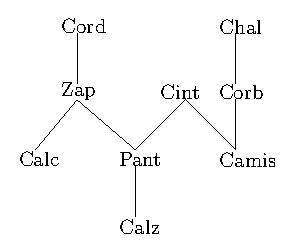
\includegraphics{eps_imgs/diagH-tareas.eps}
\caption{Diagrama de Hasse para el orden de las tareas necesarias para vestirse}
\label{fig:diagH-tareas}
\end{figure}

En este caso, el diagrama nos entrega información como por ejemplo que lo primero que se debe hacer es ponerse los calcetines, los calzoncillos o la camisa, y que lo último que se hará será abrocharse los cordones, abrocharse el cinturón o ponerse el chaleco.
Los primeros son los elementos minimales del conjunto, los segundos son los elementos maximales del conjunto.
\end{ejemplo}

\begin{definicion}
Dado un orden parcial $(A,\preceq)$, un Diagrama de Hasse para él se construye siguiendo las reglas:
\begin{enumerate}
  \itemsep 0pt
  \item Para cada elemento $x\in A$, $x$ se debe ``dibujar en el digarama''.
  \item Si $x,y\in A$ dos elementos distintos tales que $x\preceq y$, entonces x debe dibujarse ``más abajo'' que $y$ en el diagrama.
  \item Si $x,y\in A$, $x\not=y$, $x\preceq y$ y no existe ningún elemento $z$ (distinto de $x$ e $y$) tal que $x\preceq z$ y $z\preceq y$, entonces se dibuja una linea entre $x$ e $y$ en el diagrama.
\end{enumerate}
\end{definicion}

\begin{ejemplo}
Sea $\U=\{1,2,3\}$ y el orden $(\P(\U),\subseteq)$.
Su diagrama de Hasse asociado se ve en la figura~\ref{fig:diagH-subconjuntos}.

\begin{figure}[h!]
\centering
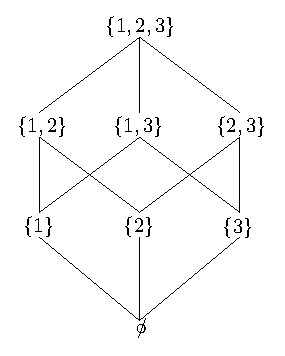
\includegraphics{eps_imgs/diagH-subconjuntos}
\caption{Diagrama de Hasse para el orden $(\P(\{1,2,3\}),\subseteq)$.}
\label{fig:diagH-subconjuntos}
\end{figure}
\end{ejemplo}

\begin{definicion}
Sea $(A,\preceq)$ un orden parcial.
Si para cualquier par de elementos $x,y\in A$ ocurre que el conjunto $\{x,y\}\subseteq A$ tiene supremo e ínfimo en $A$, diremos que $(A,\preceq)$ es un \emph{reticulado}.
Llamaremos también \emph{reticulado} a su Diagrama de Hasse asociado.
\end{definicion}

\begin{ejemplo}
El orden $(\P(\{1,2,3\}),\subseteq)$ es un reticulado.
En general, para cualquier conjunto $\U$, el orden $(\P(\U),\subseteq)$ es un reticulado,
de hecho dados $A,B\in\P(\U)$, el conjunto $\{A,B\}$ siempre tiene supremo e ínfimo, a saber \[\sup\{A,B\}=A\cup B \hspace*{3em} \inf\{A,B\}=A\cap B.\]
La demostración de estas dos últimas propiedades se deja como ejercicio.
\end{ejemplo}


\subsection{Relaciones de Equivalencia y Particiones}
\begin{definicion}
Diremos que una relación binaria $R$ sobre un conjunto $A$ es una {\bf relación de equivalencia} si cumple con ser, refleja, simétrica y transitiva.
Generalmente cuando $R$ sea una relación de equivalencia sobre $A$, la denotaremos por el símbolo $\eqr$.
Si $(x,y)\in\eqr$ o equivalentemente si $x\eqr y$ diremos que ``$x$ es equivalente a $y$''.
\end{definicion}

\begin{ejemplo}
\begin{enumerate}
  \itemsep 0pt
  \item La relación de equivalencia módulo $n$, $\equiv_n$ sobre los naturales es una relación de equivalencia.
  \item La relación $R_C$ sobre $\P(\U)$ para un $\U$ cualquiera, tal que $A,B,C\in\P(\U)$, $A R_CB\Leftrightarrow A\cap C= B\cap C$ es una relación de equivalencia.
  \item La relación $\downarrow$ sobre $\N\times\N$ definida por $(m,n)\downarrow(r,s)\Leftrightarrow m+s=n+r$, es una relación de equivalencia.

\end{enumerate}
En la sección~\ref{sec:prop-rel} demostramos las propiedades necesarias para los casos 1 y 2.
La demostración de que $\downarrow$ es también una relación de equivalencia se deja como ejercicio.
\end{ejemplo}

\begin{definicion}
Sea $A$ un conjunto cualquiera, y sea $\mathcal S$ una colección de subconjuntos de $A$ ($\mathcal S\subseteq\P(A)$).
Diremos que $\mathcal S$ es una partición de $A$ si cumple:
\begin{enumerate}
  \itemsep 0pt
  \item $\forall X\in\mathcal S$, $X\not=\emptyset$.
  \item $\bigcup\mathcal S=A$
  \item $\forall X,Y\in\mathcal S$ si $X\not=Y$ entonces $X\cap Y=\emptyset$.
\end{enumerate}
Esta definición nos dice que una partición de $A$ es una colección de conjuntos no vacíos (1) disjuntos (3) y exhaustivos (2), es decir, una colección de conjuntos no vacíos, que no comparten elementos y tal que de su unión resulta el conjunto $A$ completo.
\end{definicion}

Existe una íntima relación entre las particiones de un conjunto y las relaciones de equivalencia sobre él.
La siguiente definición nos indica la primera de estas relaciones.

\begin{definicion}
Sea $\eqr$ una relación de equivalencia cualquiera sobre un conjunto $A$.
Para cada $x\in A$ se define \emph{la clase de equivalencia de} $x$ como el conjunto $[x]_\eqr$
\[
[x]_\eqr=\{y\in A\;|\; y\eqr x\}.
\]
Cuando la relación de equivalencia (en este caso $\eqr$) esté implícita en la aplicación, a veces en vez de $[x]_\eqr$ hablaremos simplemente de $[x]$.
Una de las primeras propiedades importantes que se deben notar es que, siempre ocurre que $x\in[x]$, y que si $x\eqr y$ entonces se cumple que $[x]=[y]$ >Por qué?
\end{definicion}

\begin{ejemplo}
Tomemos la relación $\equiv_4$ sobre los naturales.
Ya sabemos que esta es una relación de equivalencia, miremos cuáles son sus clases de equivalencia:
\[
\begin{array}{l}
[0]=\{0,4,8,12,16,\ldots\} \\
\text{[}1]=\{1,5,9,13,17,\ldots\} \\
\text{[}2]=\{2,6,10,14,18,\ldots\} \\
\text{[}3]=\{3,7,11,15,19,\ldots\} \\
\end{array}
\]
Las anteriores son todas las clases de equivalencias generadas por la relación $\equiv_4$, de hecho si tomamos por ejemplo $[4]$ sabemos que $[4]=[0]$ y que $[23]=[3]$.
\end{ejemplo}

\begin{ejemplo}
Tomemos la relación $\downarrow$ sobre $\N\times\N$, las clases de equivalencia generadas son:
\[
\begin{array}{rcl}
[(0,0)]& = &\{(0,0),(1,1),(2,2),\ldots\} \\
\text{[}(0,1)]& = &\{(0,1),(1,2),(2,3),\ldots\} \\%= \{(i,j)\;|\;i+1=j\} \\
\text{[}(1,0)]& = &\{(1,0),(2,1),(3,2),\ldots\} \\%= \{(i,j)\;|\;j+1=i\}\\
\text{[}(0,2)]& = &\{(0,2),(1,3),(2,4),\ldots\} \\%= \{(i,j)\;|\;i+2=j\} \\
\text{[}(2,0)]& = &\{(2,0),(3,1),(4,2),\ldots\} \\%= \{(i,j)\;|\;j+2=i\}\\
&\vdots\\
\text{[}(0,n)]& = &\{(0,n),(1,n+1),(2,n+2),\ldots\} \\% = \{(i,j)\;|\;i+n=j\}\\
\text{[}(n,0)]& = &\{(n,0),(n+1,1),(n+2,2),\ldots\} \\%= \{(i,j)\;|\;j+n=i\}\\
&\vdots
\end{array}
\]
\vspace*{-25pt}
\end{ejemplo}


\begin{teorema}
\label{teo:equiv-rel}
Sea $\eqr$ una relación de equivalencia sobre un conjunto $A$, entonces se cumple que
\begin{enumerate}
  \itemsep 0pt
  \item $\forall x\in A$, $x\in[x]$.
  \item $x\eqr y$ si y sólo si $[x]=[y]$.
  \item si $[x]\not=[y]$ entonces $[x]\cap[y]=\emptyset$.
\end{enumerate}
\begin{demostracion}
Las primeras dos propiedades se dejan como ejercicio, demostraremos sólo la propiedad 3.
\begin{enumerate}
  \setcounter{enumi}{2}
  \item Daremos un argumento por contradicción.
  Supongamos que $[x]\not=[y]$, y supongamos que $[x]\cap[y]\not=\emptyset$, entonces necesariamente existe un $z$ tal que $z\in[x]$ y $z\in[y]$.
  Esto quiere decir que simultáneamente ocurre que $z\eqr x$ y que $z\eqr y$.
  Dado que $\eqr$ es una relación de equivalencia, cumple con ser simétrica y transitiva.
  Usando la primera de estas propiedades concluimos que $x\eqr z$ y usando esto último y la propiedad de transitividad concluimos que $x\eqr y$, luego por la porpiedad (2) se concluye que $[x]=[y]$ lo que es una contradicción.
\end{enumerate}
\end{demostracion}

De este teorema se concluye inmediatamente el siguiente.
\end{teorema}

\begin{teorema}
\label{teo:clases-equiv}
Sea $\eqr$ una relación de equivalencia sobre un conjunto $A$.
Y sea $\mathcal S$ el conjunto de las clases de equivalencia de $\eqr$, o sea $\mathcal S=\{[x]\;|\;x\in A\}$.
Entonces $S$ forma una partición de $A$.

\begin{demostracion}
Debemos demostrar las tres propiedades necesarias para que $\mathcal S$ sea una partición, a saber, que (1) es una colección de conjuntos no vacíos, (2) exhaustivos y (3) disjuntos.
En este caso, cada uno de los conjuntos de $\mathcal S$ son las clases de equivalencia de $\eqr$.
\begin{enumerate}
  \vspace*{-\topsep}
  \itemsep 0pt
  \item Debemos demostrar que $\forall X\in\mathcal S$, se tiene que $X\not=\emptyset$.
  Ahora, como los elementos de $\mathcal S$ son clases de equivalencia de $\eqr$ y dado que para todo $x$ se cumple que $x\in[x]\Rightarrow [x]\not=\emptyset$ (parte 1 del teorema~\ref{teo:equiv-rel}) entonces todos los conjuntos de $\mathcal S$ son distintos de vacío.
  \item Debemos demostrar que $\bigcup\mathcal S=A$.
  Es claro que $\bigcup\mathcal S\subseteq A$ ya que un elemento pertenece a $\bigcup\mathcal S$ si  pertenece a alguna de las clases de equivalencia de $\eqr$, y en las clases de equivalencia de $\eqr$ sólo hay elementos de $A$.
  Sólo falta demostrar entonces que $A\subseteq\bigcup\mathcal S$.
  Sea $x\in A$ sabemos que $x\in[x]$ y dado que $[x]\in\mathcal S$ concluimos que $x\in\bigcup\mathcal S$.
  \item Debemos demostrar que si $X,Y\in\mathcal S$ y $X\not=Y$ entonces $X\cap Y=\emptyset$.
  Dado que los conjuntos en $\mathcal S$ son clases de equivalencia, y por la propiedad 3 del teorema~\ref{teo:equiv-rel}, tenemos que $[x]\not=[y]$ entonces $[x]\cap[y]=\emptyset$ que es lo que queríamos demostrar.
\end{enumerate}
\end{demostracion}
\end{teorema}

\begin{definicion}
Al conjunto $\mathcal S$ del teorema anterior le llamaremos \emph{conjunto cuociente} de $A$ con respecto a $\eqr$ y lo anotaremos $A/\eqr$,
\[
A/\eqr=\{[x]\;|\;x\in A\}
\]
El teorema~\ref{teo:clases-equiv} dice entonces que si $\eqr$ es una relación de equivalencia sobre $A$, el conjunto cuociente $A/\eqr$ forma una partición de $A$.

Definiremos además el \emph{índice} de una relación de equivalencia como la cantidad de clases de equivalencias que induce, es decir, como la cantidad de elementos del conjunto cuociente $A/\eqr$.
\end{definicion}

\begin{ejemplo}
Para la relación $\equiv_4$ sobre los naturales, se tiene que el conjunto cuociente es:
\[
\begin{array}{rl}
\N/\equiv_4&=\{\{0,4,8,\ldots\},\{1,5,9,\ldots\},\{2,6,10,\ldots\},\{3,7,11,\ldots\}\} \\
&=\{[0],[1],[2],[3]\}
\end{array}
\]
El índice de la relación $\equiv_4$ sobre $\N$ es $4$ ya que induce $4$ clases de equivalencias distintas.

Para la relación $\downarrow$ sobre $\N\times\N$, se tiene que el conjunto cuociente es:
\[
(\N\times\N)/\downarrow=\{[(0,0)],[(0,1)],[(1,0)],[(0,2)],[(2,0)],[(0,3)],\ldots\}
\]
Esta relación tiene índice infinito ya que induce una cantidad infinita de clases de equivalencia.
Un diagrama de las particiones inducidas por esta relación se puede ver en la figura~\ref{fig:uparrow-equiv}.
\begin{figure}[h!]
\centering
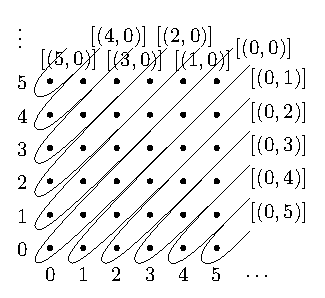
\includegraphics{eps_imgs/uparrow-equiv}
\caption{Partición de $\N\times\N$ inducida por la clase de equivalencias $\downarrow$.}
\label{fig:uparrow-equiv}
\end{figure}
\end{ejemplo}

Algo muy interesante es que a partir de una partición cualquiera de un conjunto siempre se forma una relación de equivalencia.
El siguiente teorema lo establece.

\begin{teorema}
Sea $\mathcal S$ una partición cualquiera sobre un conjunto $A$, entonces la relación $\eqr$ definida como sigue es una relación de equivalencia sobre $A$.
\[
x,y\in A,\;\;\;\;\; x\eqr y\Leftrightarrow \exists X\in\mathcal S\text{ tal que }\{x,y\}\subseteq X,
\]
o sea, $x$ está relacionado con $y$ cuando ambos pertenecen al mismo conjunto en $\mathcal S$.

\begin{demostracion}
Sólo se debe comprobar que $\eqr$ es refleja, simétrica y transitiva.
Se deja como ejercicio.
\end{demostracion}

En este caso también se cumple que $\mathcal S=A/\eqr$.
\end{teorema}

Uno de las mayores aplicaciones de las relaciones de equivalencia es que estas pueden usarse para definir nuevos conjuntos a partir del conjunto cuociente.
Veremos dos ejemplos de cómo a partir de un conjunto conocido ($\N$) pueden crearse nuevos conjuntos y definirse operaciones sobre los elementos de los nuevos conjuntos.

\begin{ejemplo}
Podemos definir el conjunto de los naturales módulo $4$, $\N_4$, como el conjunto cuociente $\N/\equiv_4$, así $\N_4=\{[0],[1],[2],[3]\}$.
Lo interesante es que podemos definir operadores en este nuevo conjunto a partir de operadores en el antiguo conjunto.
Definimos la suma módulo $4$ de la siguiente forma:
\[
[i]+_{(4)}[j]=[i+j].
\]
Así por ejemplo $[3]+_{(4)}[2]=[3+2]=[5]=[1]$, de la misma forma $[1]+_{(4)}[3]=[0]$.
También podemos definir la multiplicación módulo $4$ de la siguiente manera:
\[
[i]\cdot_{(4)}[j]=[i\cdot j].
\]
Así por ejemplo $[2]\cdot_{(4)}[3]=[2\cdot 3]=[6]=[2]$, de la misma forma $[3]\cdot_{(4)}[3]=[1]$.

Si damos un paso más y renombramos los elementos de $\N_4$ de la siguiente manera:
%manera tal que a $[0]$ le llamamos simplemente $0$, a $[1]$ le llamamos $1$, a $[2]$ le llamamos $2$, y a $[3]$ le llamamos $3$,  
\[
\begin{array}{ccc}
[0]&\leftrightarrow&0\\
\text{[} 1]&\leftrightarrow&1\\
\text{[}2]&\leftrightarrow&2\\
\text{[}3]&\leftrightarrow&3
\end{array}
\]
o sea, a $[0]$ le llamamos simplemente $0$, a $[1]$ le llamamos $1$, etc., y además reemplazamos el símbolo $+_{(4)}$ por $+$, y $\cdot_{(4)}$ por $\cdot$, tenemos un conjunto con una nueva estructura de operadores:
\[
\N_4=\{0,1,2,3\}\text{ con operadores }+\text{ y }\cdot
\]
tal que por ejemplo, $2+2=0$, $3+2=1$, $3\cdot 3=1$, $2\cdot 1=2$, etc.
\end{ejemplo}

\begin{ejemplo}
Formalmente podemos definir al conjunto de los números enteros $\Z$ como el conjunto cuociente $(\N\times\N)/\downarrow$, así formalmente $\Z=\{[(0,0)],[(0,1)],[(1,0)],[(0,2)],[(2,0)],[(0,3)],\ldots\}$.
Intuitivamente la clase de equivalencia $[(0,i)]$ está representando al entero $i$, y la clase de equivalencia $[(i,0)]$ está representando al entero $-i$.
Entonces podemos renombrar los elementos de este conjunto de la siguiente manera:
\[
\begin{array}{ccr}
\text{[}(0,0)]&\leftrightarrow&0\\
\text{[}(0,1)]&\leftrightarrow&1\\
\text{[}(1,0)]&\leftrightarrow&-1\\
\text{[}(0,2)]&\leftrightarrow&2\\
\text{[}(2,0)]&\leftrightarrow&-2\\
\text{[}(0,3)]&\leftrightarrow&3\\
&\vdots
\end{array}
\]
luego $\Z=\{0,1,-1,2,-2,3,-3,4\ldots\}$.
Lo primero (importante) que notar es que ``$-1$'' es {\bf simplemente un nombre} que se le da a la clase $[(1,0)]$, así como ``$-2$'' a la clase $[(2,0)]$, no debe interpretarse el símbolo ``$-$'' con ningún significado especial, de hecho en nuestro caso ``$-$'' no significa nada por sí sólo.

Podemos intentar definir operadores sobre este nuevo conjunto de manera similar al ejemplo anterior, teniendo la intuición de que estos deben captar la estructura de $\Z$.
Por ejemplo podríamos definir el operador $+_\downarrow$ de la siguiente forma:
\[
[(m,n)]+_\downarrow[(r,s)]=[(m+r,n+s)],
\]
así se tendría que $[(0,7)]+_\downarrow[(5,0)]=[(5,7)]=[(0,2)]$, que $[(18,0)]+_\downarrow[(0,4)]=[(18,4)]=[(14,0)]$, y que $[(3,0)]+_\downarrow[(6,0)]=[(9,0)]$, etc.,
lo que capta completamente la idea de la suma entera, de hecho resulta que $7+_\downarrow-5=2$, $-18+_\downarrow 4=-14$ y $-3+_\downarrow-6=-9$.

Para definir la multiplicación debemos cuidarnos un poco más, de hecho una definición como la siguiente no nos lleva a buen término
\[
[(m,n)]\cdot_\downarrow[(r,s)]=[(m\cdot r,n\cdot s)],
\]
ya que por ejemplo nos resulta que $[(3,0)]\cdot_\downarrow[(4,0)]=[(3\cdot 4,0\cdot 0)]=[(12,0)]$ o sea que $-3\cdot_\downarrow-4=-12$ cuando quisiéramos que el resultado fuese $12$.
La definición correcta de $\cdot_\downarrow$ es:
\[
[(m,n)]\cdot_\downarrow[(r,s)]=[(m\cdot s+n\cdot r,m\cdot r+n\cdot s)].
\]
De hecho ahora resulta que $[(3,0)]\cdot_\downarrow[(4,0)]=[(3\cdot 0+0\cdot 4,3\cdot 4+0\cdot 0)]=[(0,12)]$, y que $[(0,3)]\cdot_\downarrow[(0,3)]=[(0\cdot 3+3\cdot 0,0\cdot 0+3\cdot 3)]=[(0,9)]$, etc., lo que capta la idea de multiplicación entera ya que $-3\cdot_\downarrow-4=12$ y $3\cdot_\downarrow 3=9$.

Luego podemos usar el conjunto $\Z=\{0,1,-1,2,-2,3,\ldots\}$ y renombrar las operaciones $+_\downarrow$ y $\cdot_\downarrow$ como $+$ y $\cdot$ simplemente para obtener a los enteros y sus dos operaciones habituales.
\end{ejemplo}
